\section[Theorie]{Theorie \textnormal{\cite{faraday}}}
\label{sec:theorie}

Nichtrelativistische Quantensysteme werden durch die Schrödingergleichung beschrieben. Die Dynamik eines Teilchens der
Masse $m$ im Zustand $\bm{\Psi}$ nimmt dann die Form
\begin{align*}
    E \bm{\Psi} = H \bm{\Psi} = \pfrac{p^2}{2m} \bm{\Psi} + V \bm{\Psi} = \pfrac{\hbar^2 k^2}{2m} \bm{\Psi} + V \bm{\Psi}
\end{align*}
an, wobei $E$ die Energie, $p$ den Impuls und $k$ die Wellenzahl beschreiben. Mit $\hbar$ wird die reduzierte Planckkonstante
bezeichnet. Für den freien Grenzfall mit verschwindendem Potential $V$ weisen Energieeigenzustände demnach
eine parabolische Dispersion
\begin{align*}
    E(k) = \pfrac{\hbar^2 k^2}{2m} %\tag{1a}\label{eqn:frei}
\end{align*}
auf. Im für die in Festkörpern auftretende Gitterperiodizität konzipierten reduzierten Zonenschema folgen diese Funktionen
den erlaubten Energiebändern der Gitterelektronen. Unter der Annahme freier Elektronen entstehen dann Entartungen am Zonenrand.

\subsection{Bandstruktur}

Durch die strukturelle Anordnung der Gitteratome wirkt im Festkörper ein periodisches Potential, das für ein Auflösen der
Energieentartung der Elektronen sorgt. Stattdessen bilden sich Bandlücken aus, deren Energiebereiche nicht besetzt werden
können. Die Beschreibung als freie Teilchen ist nun ebenfalls nicht mehr gültig. Für schwach gebundene Elektronen kann
$E(k)$ allerdings um ein Minimum $E'(k_0) = 0$ in $k$ entwickelt werden. Bis zur quadratischen Ordnung ergeben die ersten
Glieder der Potenzreihe
\begin{align*}
    E(k) \approx E(k_0) + E'(k_0) (k - k_0) + \pfrac{1}{2} E''(k_0) (k - k_0)^2 = E(k_0) + \pfrac{1}{2} E''(k_0) (k - k_0)^2
\end{align*}
und vereinfachen sich mit der Auswahl $E(k_0) \equiv 0$ und $k_0 \equiv 0$ zu
\begin{align*}
    E(k) \approx \pfrac{1}{2} E''(0) k^2
\end{align*}
als parabolische Näherung. Dieser Ausdruck lässt sich analog zum vollständig freien Grenzfall als
\begin{align*}
    E(k) \approx \pfrac{\hbar^2 k^2}{2m^{*}} %\tag{1b}\label{eqn:quasi}\stepcounter{equation}
\end{align*}
formulieren. \enlargethispage{\baselineskip}\pagebreak

An dieser Stelle definieren wir den Ausdruck
\begin{align}
    m^{*} = \hbar^2 \left( \pfrac{\del^2 E}{\del k^2} \right)^{\!\! -1} \label{eqn:effektiv}
\end{align}
als effektive Masse. Die Interpretation dieser Schreibweise besagt also, dass sich quasifreie Elektronen in zweiter Ordnung
wie freie Ladungsträger mit Masse $m^{*}$ verhalten. Damit Abweichungen in verschiedene Raumrichtungen vernachlässigbar sind,
wird ein hinreichend hoher Grad an Symmetrie vom Kristall gefordert.

\begin{figure}[H]
    \vspace{1ex}
    \centering
    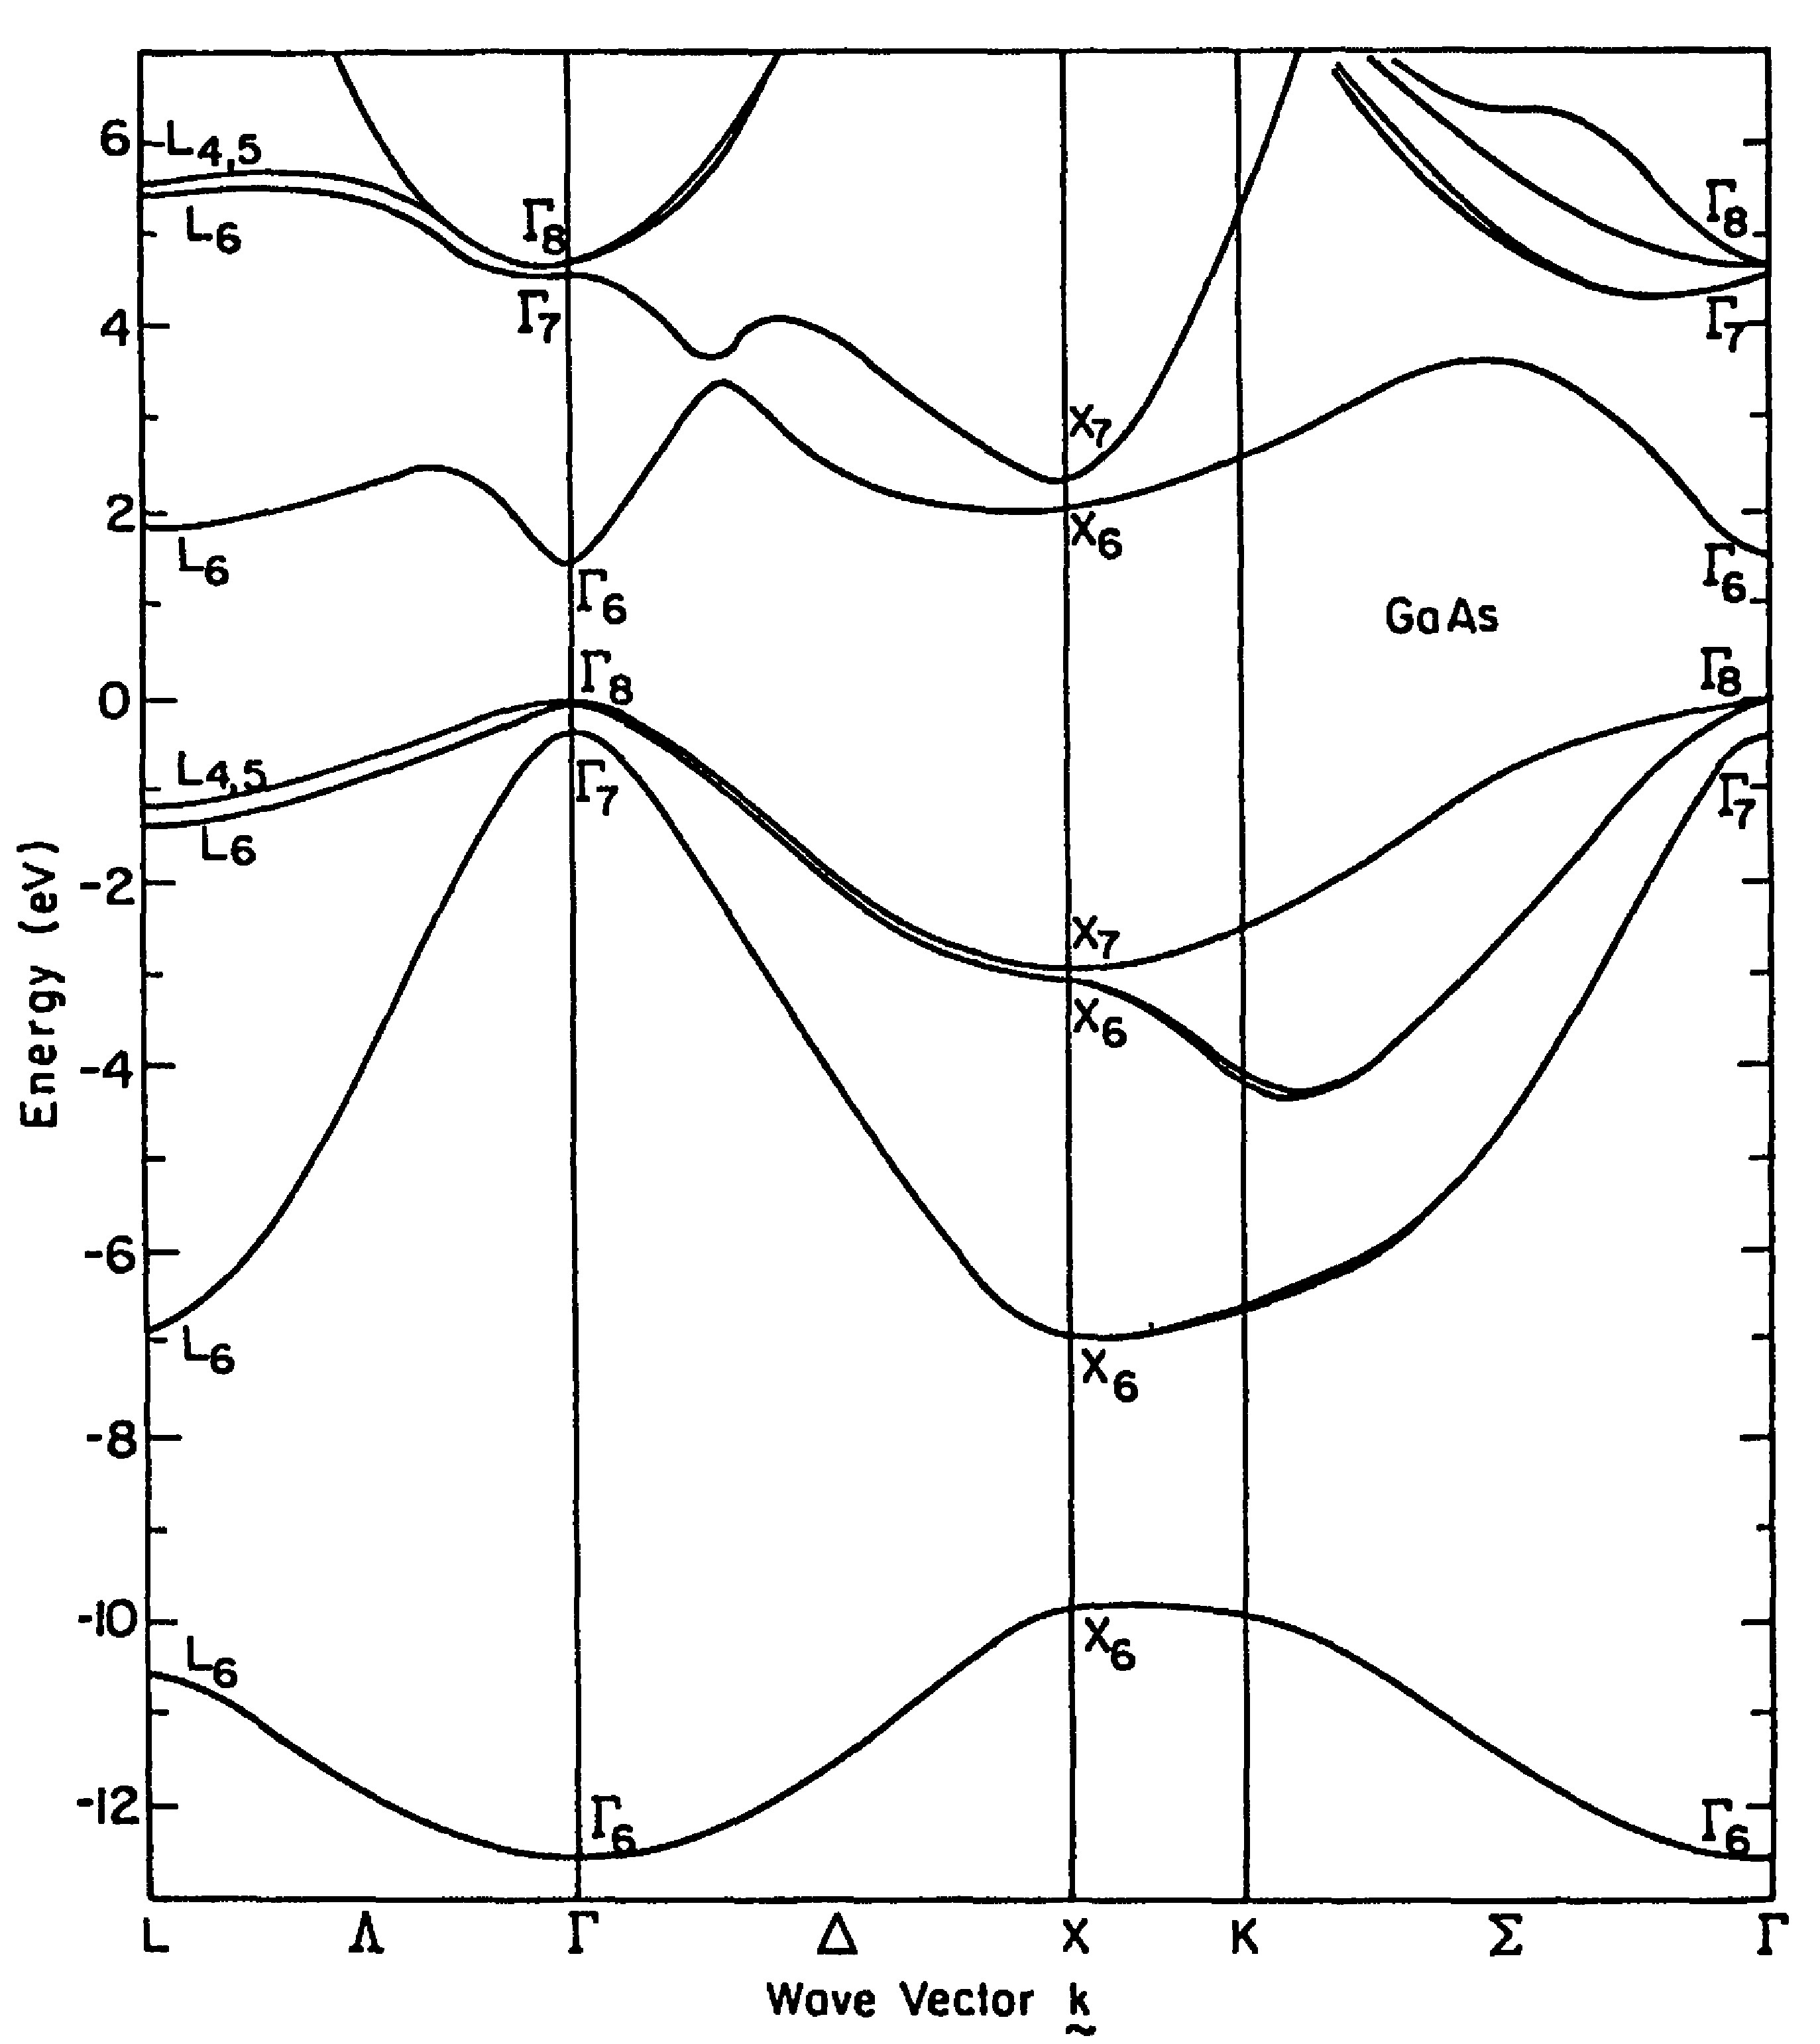
\includegraphics[width=0.55\textwidth]{content/grafik/bandstruktur.jpg}
    \caption{Berechnete Bandstruktur von GaAs um die Bandlücke. \cite{coh_jam_el}}
    \label{fig:band}
\end{figure}

Abbildung~\ref{fig:band} zeigt exemplarische Bandverläufe für reines GaAs. Neben dem Auftreten von Bandlücken lässt sich auch
die lokal parabolische Form der Elektronendispersion deutlich erkennen. Unsere Approximation erscheint damit gerechtfertigt.

Zur Charakterisierung wesentlicher Materialeigenschaften von Festkörpern ist es sinnvoll, die Begriffe Valenzband~(VB) und
Leitungsband~(LB) einzuführen. Bei einer absoluten Temperatur $T = 0$ gibt das VB den höchsten vollständig gefüllten
Energiebereich an, während das LB den niedrigsten wenigstens teilweise oder auch vollständig unbesetzten Bereich umfasst.
In dieser Betrachtung ist ein Stoff gerade dann leitfähig, wenn sich ausreichend viele Elektronen im LB befinden. 

Im gegebenen Kontext sollte zur Einordnung verschiedener Materialklassen außerdem die Fermienergie~$E_F$ erwähnt werden.
Am absoluten Temperaturnullpunkt sind laut der Fermi-Dirac Verteilung alle niedrigeren Zustände $E < E_F$ besetzt
und alle höheren Zustände $E > E_F$ unbesetzt. \enlargethispage{\baselineskip}\pagebreak

Durch Erwärmung wird diese Trennung zunehmend unscharf. Da viele relevante Festkörper eine über die Boltzmannkonstante~$k_B$
und $E_F = k_B T_F$ definierte Fermitemperatur~$T_F$~weit oberhalb des Schmelzpunktes besitzen, wird $T = 0$ hier als
Näherung beibehalten.

\begin{figure}[H]
    \vspace{3ex}
    \centering
    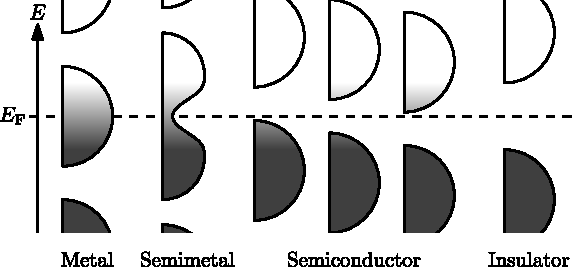
\includegraphics[width=0.7\textwidth]{content/grafik/bandstructure.pdf}
    \caption{Energieschemata verschiedener Materialklassen im Vergleich. \cite{wiki_band}}
    \label{fig:schema}
\end{figure}

In Abbildung~\ref{fig:schema} sind einige mögliche Konfigurationen von VB (unten) und LB (oben) in Relation zu $E_F$
schematisch aufgeführt. Für Metalle und Halbmetalle liegt $E_F$ innerhalb des LB, sodass solche Stoffe elektrischen Strom
gut leiten. Auf der anderen Seite besitzen Isolatoren eine große Bandlücke von mehreren \unit{\electronvolt}
zwischen VB und LB, welche auch $E_F$ enthält. Da selbst für hohe Temperaturen kaum Elektronen das LB erreichen, sind
enstsprechende Stoffe nichtleitend. Zwischen diesen Kategorien lassen sich die sogenannten Halbleiter einordnen. Sie
weisen zwar ebenfalls eine Bandlücke um $E_F$ auf, allerdings fällt diese mit wenigen \unit{\electronvolt} vergleichsweise
klein aus. Dank der niedrigeren Energiedifferenz können bereits bei moderaten Temperaturen signifikante Zahlen an Elektronen
in das LB aufsteigen, sodass sich die Leitungseigenschaften des Materials leicht ändern lassen.

\subsection{Dotierung}

Die Kategorie der Halbleiter wird nach Abbildung~\ref{fig:schema} in drei Unterkategorien eingeteilt. Bei intrinsischen
Halbleitern (mittig) handelt es sich um Reinstoffe, welche die zuvor beschriebenen Eigenschaften erfüllen. Daneben kann
die Leitfähigkeit von Materie aber auch durch gezieltes Einbringen von Fremdatomen präzise angepasst werden. Ein solches
Vorgehen wird Dotierung genannt, die resultierenden Mischstoffe werden je nach Art als Halbleiter vom p\hspace{0.25ex}-Typ
(links) oder n\hspace{0.15ex}-Typ (rechts) bezeichnet. 

Bei der n\hspace{0.15ex}-Dotierung werden Atome mit Elektronenüberschuss als Donatoren eingebracht. Die zusätzlichen
negativen Ladungen besitzen Energien knapp unterhalb des LB, sodass der Abstand zwischen LB und $E_F$ stark reduziert
wird.

Zur p\hspace{0.25ex}-Dotierung werden dagegen Atome mit Elektronendefizit als Akzeptoren verwendet. Die Energien
der zusätzlichen als Löcher bezeichneten positiven Ladungen liegen knapp oberhalb des VB, sodass die Lücke zwischen VB und
$E_F$ stark reduziert wird.

Beide Methoden steigern die Konduktivität des Halbleiters, indem insgesamt weniger Energie aufzuwenden ist, um Elektronen
ins LB zu heben. 

\subsection{Faraday-Effekt}

Der Faraday-Effekt bezeichnet das Auftreten einer Rotation der Polarisationsrichtung von linear polarisierten elektromagnetischen
Wellen beim Durchlaufen eines von einem homogenen Magnetfeld durchdrungenen transparenten Festkörpers in Richtung der Feldlinien.
Abbildung~\ref{fig:drehung} stellt dieses Phänomen für den allgemeinen Fall dar.

\begin{figure}[H]
    \vfill{2ex}
    \centering
    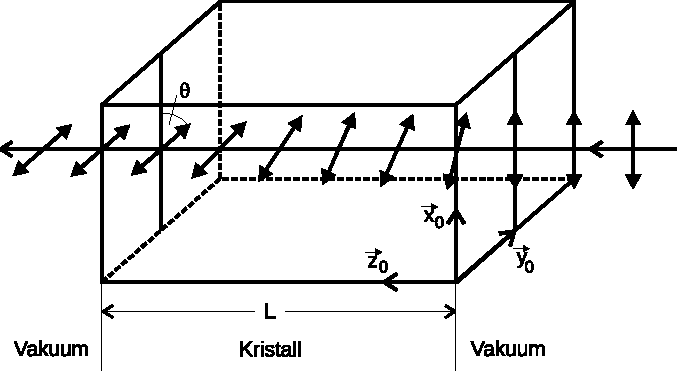
\includegraphics[width=0.7\textwidth]{content/grafik/drehung.pdf}
    \captionsetup{width=.95\linewidth}
    \caption{Drehung der Polarisationsebene beim Durchgang durch einen Kristall. \cite{faraday}}
    \label{fig:drehung}
\end{figure}

\subsubsection{Zirkulare Doppelbrechung}

Die beobachtete Drehung der Schwingungsebene bei Transmission lässt sich erklären, indem für linksgerichtet und rechtsgerichtet
polarisierte Lichtwellen jeweils abweichende Phasengeschwindigkeiten vorrausgesetzt werden. Das elektrische Feld lässt sich dann zu
\begin{align*}
    \bm{E}(z) = \pfrac{1}{2} \left(\bm{E}_R(z) + \bm{E}_L(z)\right)
\end{align*}
zerlegen, wobei die einzelnen Komponenten
\begin{align*}
    \bm{E}_R(z) &= E_0 \left(\bm{\hat{x}} - i \bm{\hat{y}}\right) e^{ik_Rz} %\tag{3a}\label{eqn:rpol} \\
    \bm{E}_L(z) &= E_0 \left(\bm{\hat{x}} + i \bm{\hat{y}}\right) e^{ik_Lz} %\tag{3b}\label{eqn:lpol}\stepcounter{equation}
\end{align*}
lauten. Daraus kann beim Eintritt ins Material an der Stelle $z = 0$ direkt
\begin{align}
    \bm{E}(0) = E_0 \bm{\hat{x}} \label{eqn:eintritt}
\end{align}
abgelesen werden. \enlargethispage{\baselineskip}\pagebreak

Nachdem die Länge des Festkörpers $L$ zurückgelegt ist, gibt
\begin{align*}
    \bm{E}(L) = \pfrac{1}{2} E_0 \left( 
                \left( e^{ik_RL} + e^{ik_LL} \right) \bm{\hat{x}} +
                \left( e^{ik_RL} - e^{ik_LL} \right) \bm{\hat{y}} \right)
\end{align*}
die Feldstärke an. Durch Einführen der Hilfsgrößen
\begin{align}
    \psi &\equiv \pfrac{L}{2} (k_R + k_L) \nonumber \\
    \theta &\equiv \pfrac{L}{2} (k_R - k_L) \label{eqn:theta_a}
\end{align}
lässt sich dieser Term zu
\begin{align*}
    \bm{E}(L) = \pfrac{1}{2} E_0 \left( 
                \left( e^{i\psi}e^{i\theta} + e^{i\psi}e^{-i\theta} \right) \bm{\hat{x}} +
                \left( e^{i\psi}e^{i\theta} - e^{i\psi}e^{-i\theta} \right) \bm{\hat{y}} \right)
\end{align*}
umschreiben, mit der eulerschen Formel $e^{ia} = \cos a + i \sin a$ wird daraus
\begin{align*}
    \bm{E}(L) = E_0 e^{i\psi} (\cos\theta \,\bm{\hat{x}} + \sin\theta \,\bm{\hat{y}})
\end{align*}
beim Austritt aus dem Material. Im Vergleich mit~\eqref{eqn:eintritt} wird deutlich, dass es sich hierbei wieder um eine
linear polarisierte Welle handelt, die um einen Winkel $\theta$ gedreht schwingt. 

Mithilfe der Definition für Phasengeschwindigkeit
\begin{align*}
    v = \pfrac{\omega}{k}
\end{align*}
und Brechungsindex
\begin{align*}
    n = \pfrac{c}{\raisebox{0.5ex}{$v$}} = \pfrac{ck}{\raisebox{0.5ex}{$\omega$}}
\end{align*}
lässt sich~\eqref{eqn:theta_a} als
\begin{align*}
    \theta = \pfrac{L\omega}{2c} (n_R - n_L)
\end{align*}
formulieren. Dabei beschreibt $c$ die Vakuumslichtgeschwindigkeit.

Zirkulare Doppelbrechung tritt als Konsequenz induzierter elektrischer Dipolmomente auf, die eine makroskopische
Gesamtpolarisation $\bm{P}$ erzeugen. Für kleine Feldstärken $\bm{E}$ kann diese mit der Influenzkonstanten $\varepsilon_0$
über $\bm{P} \approx \varepsilon_0 \bm{\chi E}$ aufgestellt werden. Im isotropen Medium wird die dielektrische Suszeptibilität
$\bm{\chi}$ skalar, für den anisotropen Fall muss sie als Tensor aufgefasst werden. Bei ordinärer Brechung gibt
\begin{align*}
    \bm{\chi} = \begin{pmatrix}
        \chi_{xx} & 0 & 0 \\
        0 & \chi_{yy} & 0 \\
        0 & 0 & \chi_{zz} \end{pmatrix}
\end{align*}
die Schreibweise von $\bm{\chi}$ als diagonale Matrix nach Hauptachsentransformation an.

Um Doppelbrechung zu erzeugen, muss $\bm{\chi}$ die Form einer nichtdiagonalen hermiteschen Matrix annehmen.
Der einfachste Fall ist mit
\begin{align*}
    \bm{\chi} = \begin{pmatrix}
        \chi_{xx} & i\chi_{xy} & 0 \\
        -i\chi_{xy} & \chi_{xx} & 0 \\
        0 & 0 & \chi_{zz} \end{pmatrix}
\end{align*}
gegeben, wobei gleichartige Brechung in der Normalenebene zur Ausbreitungsrichtung angesetzt wird. Im folgenden zeigen wir,
dass aus dieser Formulierung verschiedene Wellenvektoren für beide Polarisationsanteile folgen.

Zur Beschreibung der Welle in Materie wird die dielektrische Verschiebung
\begin{align}
    \bm{D} = \varepsilon_0 \bm{E} + \bm{P} \approx \varepsilon_0 (\bm{1 + \chi}) \bm{E} \label{eqn:verschiebung}
\end{align}
verwendet. Weiter ergibt sich aus den Maxwellgleichungen sowie der Relation zwischen magnetischer Flussdichte $\bm{B}$ und
Feldstärke $\bm{H}$ 
\begin{align*}
    \bm{\nabla} \times (\bm{\nabla} \times \bm{E}) = -\bm{\nabla} \times \pfrac{\partial \bm{B}}{\partial t} =
    -\mu_0 \pfrac{\partial}{\partial t} \bm{\nabla} \times \bm{H} = -\mu_0 \pfrac{\partial}{\partial t}
    \left( \bm{j} + \pfrac{\partial \bm{D}}{\partial t} \right)
\end{align*}
und indem~\eqref{eqn:verschiebung} verwendet wird
\begin{align*}
    \bm{\nabla} \times (\bm{\nabla} \times \bm{E}) \approx -\mu_0 \pfrac{\partial^2 \bm{D}}{\partial t^2} \approx
    -\varepsilon_0 \mu_0 (\bm{1 + \chi}) \pfrac{\partial^2 \bm{E}}{\partial t^2} =
    -\pfrac{1}{c^2} (\bm{1 + \chi}) \pfrac{\partial^2 \bm{E}}{\partial t^2}
\end{align*}
unter Vernachlässigung der Stromdichte $\bm{j}$ gegenüber der Änderung der Polarisation. Mit dem Ansatz einer ebenen Welle
mit $\bm{k}$ als Wellenvektor und $\omega$ als Kreisfrequenz
\begin{align*}
    \bm{E} = \bm{E}_0 e^{i(\bm{kr} - \omega t)}
\end{align*}
folgt nach Ausführen der Differentialoperatoren
\begin{align}
    \bm{k} \times (\bm{k} \times \bm{E}) \approx -\pfrac{\omega^2}{c^2} (\bm{1 + \chi}) \bm{E} \label{eqn:näherung}
\end{align}
als Näherungsergebnis. Durch Koordinatenwahl
\begin{align*}
    \bm{k} = k\bm{\hat{z}}
\end{align*}
und
\begin{align*}
    \bm{E} = E_x \bm{\hat{x}} + E_y \bm{\hat{y}} + E_z \bm{\hat{z}}
\end{align*}
kann außerdem
\begin{align*}
    \bm{k} \times (\bm{k} \times \bm{E}) = -k^2 (E_x \bm{\hat{x}} + E_y \bm{\hat{y}})
\end{align*}
für die linke Seite von~\eqref{eqn:näherung} geschrieben werden.

Ausführen des Matrixprodukts liefert
\begin{align*}
    \bm{\chi E} = (\chi_{xx}E_x + i\chi_{xy}E_y) \bm{\hat{x}} + (\chi_{xx} E_y - i \chi_{xy}E_x) \bm{\hat{y}} +
    \chi_{zz} E_z \bm{\hat{z}} 
\end{align*}
für die rechte Seite von~\eqref{eqn:näherung} und erlaubt für die Komponente in Ausbreitungsrichtung
\begin{align*}
    \pfrac{\omega^2}{c^2} (1 + \chi_{zz}) E_z \approx 0
\end{align*}
direkt die Aussage, dass die Welle wegen
\begin{align*}
    E_z \approx 0
\end{align*}
transversal schwingt. Die dazu orthogonalen Komponenten können anhand~\eqref{eqn:näherung} leicht als homogenes lineares Gleichungssystem
\begin{align}
    \bm{C} \begin{pmatrix} E_x \\ E_y \end{pmatrix} = \begin{pmatrix}
    \pfrac{\omega^2}{c^2} (1 + \chi_{xx}) - k^2 & i\pfrac{\omega^2}{c^2} \chi_{xy} \\
    i\pfrac{\omega^2}{c^2} \chi_{xy} & -\pfrac{\omega^2}{c^2} (1 + \chi_{xx}) + k^2 \end{pmatrix}
    \begin{pmatrix} E_x \\ E_y \end{pmatrix} \approx \begin{pmatrix} 0 \\ 0 \end{pmatrix} \label{eqn:system}
\end{align}
zusammengefasst werden. Damit dieses eine nichtriviale Lösung besitzt, muss zwingend die Determinante der Koeffizientenmatrix
\begin{align*}
    0 = -\det \bm{C} = \left( \pfrac{\omega^2}{c^2} (1 + \chi_{xx}) - k^2 \right)^{\!\! 2} + i^2 \pfrac{\omega^4}{c^4} \chi_{xy}^2
\end{align*}
verschwinden. Es ergeben sich zwei Lösungen
\begin{align}
    k_{\pm} = \pfrac{\omega}{\raisebox{0.5ex}{$c$}} \sqrt{1 + \chi_{xx} \pm \chi_{xy}} \label{eqn:wellenzahl}
\end{align}
für die Wellenzahl und somit
\begin{align*}
    v^R_L = \pfrac{c}{\sqrt{1 + \chi_{xx} \pm \chi_{xy}}}
\end{align*}
für die Phasengeschwindigkeit, die entweder größer oder kleiner als 
\begin{align}
    v = \pfrac{c}{\sqrt{1 + \chi_{xx}}} \label{eqn:geschwindigkeit}
\end{align}
für den Fall $\chi_{xy} = 0$ ist. Einsetzen von~\eqref{eqn:wellenzahl} in~\eqref{eqn:system} liefert
\begin{align}
    (E_x)^R_L = \pm \, i E_y
\end{align}
und belegt damit die Behauptung, dass sich je eine rechtszirkular und eine linkszirkular polarisierte Welle mit unterschiedlichen
Phasengeschwindigkeiten überlagern, um beim Wiedereintritt ins Vakuum eine zur initialen Ausrichtung gedrehte linear
polarisierte Welle zu bilden.

Aus Einsetzten von~\eqref{eqn:wellenzahl} in~\eqref{eqn:theta_a} folgt
\begin{align*}
    \theta = \pfrac{L}{2} (k_{+} - k_{-}) = \pfrac{L\omega}{2c} \left( \sqrt{1 + \chi_{xx} + \chi_{xy}} -
    \sqrt{1 + \chi_{xx} + \chi_{xy}} \right)
\end{align*}
als Bestimmungsformel für den Drehwinkel. Allgemein darf $\chi_{xy} \ll \chi_{xx}$ angenommen werden, sodass eine
Reihenentwicklung bis zum linearen Glied
\begin{align}
    \theta \approx \pfrac{L\omega}{2c\sqrt{1 + \chi_{xx}}} \chi_{xy} = \pfrac{L\omega v}{2c^2} \chi_{xy} =
    \pfrac{L\omega}{2cn} \chi_{xy} \label{eqn:theta_b}
\end{align}
eine gute Näherung liefert. Zur Berechnung von $\theta$ aus experimentell zugänglichen Größen muss jetzt nur noch $\chi_{xy}$
gefunden werden.

\subsubsection{Rotationswinkel}

Optisch inaktive Materialien werden erst durch Anlegen eines äußeren Magnetfeldes $\bm{B}$ doppelbrechend. Um diesen Effekt
genauer zu untersuchen, stellen wir mit
\begin{align*}
    m \pfrac{\del^2 \bm{r}}{\del t^2} + K \bm{r} = -e_0\bm{E} - e_0\pfrac{\del \bm{r}}{\del t} \times \bm{B}
\end{align*}
ein einfaches Modell für die gebundenen Gitterelektronen auf. Hier geben $\bm{r}$ die Auslenkung zur Gleichgewichtslage, $K$ eine
Kopplungskonstante der linearen Rückstellkraft und $\bm{E}$ die Feldstärke der einfallenden Lichtwelle an. Die Elementarladung wird
mit $e_0$ bezeichnet. Geschwindigkeitsproportionale Dämpfungseffekte sowie die magnetische Komponente der Welle tragen nur schwach
bei und werden daher nicht berücksichtigt. Zusammenfassend lassen sich Elektronen also als geladene harmonische Oszillatoren unter
dem Einfluss der klassischen Kräfte nach Coulomb und Lorentz auffassen.

Wir nehmen wieder eine oszillatorische Zeitabhängigkeit für das Feld an und fordern, dass die Ladungen proportional dazu
ausgelenkt werden. Einsetzen von
\begin{align*}
    \bm{E} \sim \bm{r} \sim e^{-i\omega t}
\end{align*}
erlaubt das Auflösen der Differentialoperatoren und liefert
\begin{align*}
    -m\omega^2 \bm{r} + K\bm{r} = -e_0\bm{E} + i e_0 \omega \bm{r} \times \bm{B}
\end{align*}
als Umformulierung. Aufgrund der vergleichsweise hohen Frequenz tritt mit
\begin{align*}
    \bm{P} = -Ne\bm{r}
\end{align*}
ausschließlich eine Verschiebungspolarisation auf, wobei $N$ die Anzahl der Elektronen pro Volumeneinheit angibt.
Durch Eliminieren von $\bm{r}$ lässt sich damit
\begin{align*}
    -m\omega^2 \bm{P} + K\bm{P} = Ne^2\bm{E} + i e_0 \omega \bm{P} \times \bm{B}
\end{align*}
aufstellen. \enlargethispage{\baselineskip}\pagebreak

Mit der vereinfachten Annahme eines homogenen äußeren Feldes
\begin{align*}
    \bm{B} = B \bm{\hat{z}}
\end{align*}
gibt die Komponentenschreibweise
\begin{align*}
    (K - m\omega^2) P_x &= Ne_0^2 E_x + i e_0 \omega P_y B \\
    (K - m\omega^2) P_y &= Ne_0^2 E_y - i e_0 \omega P_x B \\
    (K - m\omega^2) P_z &= Ne_0^2 E_z
\end{align*}
ein Gleichungssystem vor. Um daraus eine nichttriviale Lösung unabhängig von den Feldstärkekomponenten zu erhalten, muss
für den Suszeptibilitätstensor ein Ansatz mit imaginären nichtdiagonalen Einträgen gewählt werden. Die Trivialität der
dritten Komponente führt zu
\begin{align*}
    \bm{\chi} = \begin{pmatrix}
        \chi_{xx} & i\chi_{xy} & 0 \\
        i\chi_{yx} & \chi_{xx} & 0 \\
        0 & 0 & \chi_{zz} \end{pmatrix}
\end{align*}
als einfachste Variante. Für die erste Komponente folgt dann
\begin{align*}
    \varepsilon_0 (K - m\omega^2)(\chi_{xx}E_x + i\chi_{xy}E_y) = Ne_0^2 E_x +
    i \varepsilon_0 e_0 \omega (i\chi_{yx} E_x + \chi_{xx} E_y) B
\end{align*}
und
\begin{align}
    \varepsilon_0 (K - m\omega^2)\chi_{xx} &= Ne_0^2 - \varepsilon_0 e_0 \omega \chi_{yx}B \tag{11a}\label{eqn:komp_1a}\\
    \varepsilon_0 (K - m\omega^2)\chi_{xy} &= \varepsilon_0 e_0 \omega \chi_{xx}B \tag{11b}\label{eqn:komp_1b}\stepcounter{equation}
\end{align}
durch Vergleich von Realteilen und Imaginärteilen. Für die zweite Komponente gilt
\begin{align*}
    \varepsilon_0 (K - m\omega^2)(i\chi_{yx}E_x + \chi_{xx}E_y) = Ne_0^2 E_y -
    i \varepsilon_0 e_0 \omega (\chi_{xx} E_x + i\chi_{xy} E_y) B
\end{align*}
und
\begin{align}
    \varepsilon_0 (K - m\omega^2)\chi_{xx} &= Ne_0^2 + \varepsilon_0 e_0 \omega \chi_{xy}B \tag{12a}\label{eqn:komp_2a} \\
    \varepsilon_0 (K - m\omega^2)\chi_{yx} &= -\varepsilon_0 e_0 \omega \chi_{xx}B \tag{12b}\label{eqn:komp_2b}\stepcounter{equation}
\end{align}
aus erneutem Koeffizientenvergleich. Betrachtung der Gleichungspaare~\eqref{eqn:komp_1a} und~\eqref{eqn:komp_2a}~oder
\eqref{eqn:komp_1b} und~\eqref{eqn:komp_2b} lässt erkennen, dass
\begin{align*}
    \chi_{xy} = -\chi_{yx}
\end{align*}
erfüllt sein muss. Einsetzen erlaubt die Herleitung von
\begin{align*}
    \chi_{xy} = \pfrac{N e_0^3 \omega B}{\varepsilon_0 \left( (K - m\omega^2)^2 - (e_0\omega B)^2 \right)}
\end{align*}
für den gesuchten Ausdruck. \enlargethispage{\baselineskip}\pagebreak

Der Rotationswinkel lässt sich dann nach~\eqref{eqn:theta_b} zu
\begin{align*}
    \theta \approx \pfrac{LN e_0^3 \omega^2 B}{2\varepsilon_0 c n \left( (K - m\omega^2)^2 - (e_0\omega B)^2 \right)} =
    \frac{LN e_0^3 \omega^2 B}{2\varepsilon_0 c m^2 \left( \!\left( \pfrac{K}{m} - \omega^2 \right)^{\!\! 2} - 
    \pfrac{e_0^2 B^2}{m^2} \omega^2 \right)}
\end{align*}
abschätzen. Darin lassen sich die Resonanzfrequenz
\begin{align*}
    \omega_0 \equiv \sqrt{\pfrac{K}{\raisebox{0.5ex}{$m$}}}
\end{align*}
und die Zyklotronfrequenz
\begin{align*}
    \omega_c \equiv \frac{e_0 B}{\raisebox{0.5ex}{$m$}}
\end{align*}
identifizieren, mit deren Hilfe sich der Ausdruck zu
\begin{align*}
    \theta \approx \frac{LN e_0^3 \omega^2 B}{2\varepsilon_0 c m^2 \left( ( \omega_0^2 - \omega^2 )^2 - 
    \omega_C^2 \,\omega^2 \right)}
\end{align*}
vereinfacht. Typischerweise gilt im Experiment
\begin{align*}
    \omega_0^2 - \omega^2 \gg \omega_C \,\omega
\end{align*}
und erlaubt das Schreiben von
\begin{align*}
    \theta \approx \frac{LN e_0^3 \omega^2 B}{2\varepsilon_0 c m^2 ( \omega_0^2 - \omega^2 )^2}
\end{align*}
als weitere Vereinfachung. Über die Beziehung
\begin{align*}
    \omega = 2\pi \nu = 2\pi \pfrac{c}{\lambda}
\end{align*}
kann der Winkel auch in Abhängigkeit zur Wellenlänge $\lambda$ definiert werden.

Bei Messfrequenzen $\omega \ll \omega_0$ gilt
\begin{align*}
    \theta \approx \frac{LN e_0^3 \omega^2 B}{2\varepsilon_0 c m^2 \omega_0^4} = 
    \frac{2\pi^2 LN e_0^3 cB}{\varepsilon_0 m^2 \lambda^2 \omega_0^4}
\end{align*}
und für $\omega \gg \omega_0$ wiederum
\begin{align*}
    \theta \approx \frac{LN e_0^3 B}{2\varepsilon_0 c m^2 \omega^2} = 
    \frac{LN e_0^3 \lambda^2 B}{8\pi^2 \varepsilon_0 c^3 m^2 n}
\end{align*}
als finale Näherung. Letzterer Fall beschreibt die Problemstellung quasifreier Elektronen am besten. Die Vorschrift
\begin{align}
    \pfrac{\theta}{L} \approx \frac{N e_0^3 B}{2\varepsilon_0 c m^{*2} \omega^2} = 
    \frac{N e_0^3 \lambda^2 B}{8\pi^2 \varepsilon_0 c^3 m^{*2} n} \label{eqn:ausgleichsrechnung}
\end{align}
erlaubt uns also, die in~\eqref{eqn:effektiv} definierte effektive Elektronenmasse mit guter Genauigkeit
und unabhängig von der Ausdehnung der Probe zu bestimmen.
